\documentclass{ximera}

%\usepackage{todonotes}

\newcommand{\todo}{}

\usepackage{tkz-euclide}
\tikzset{>=stealth} %% cool arrow head
\tikzset{shorten <>/.style={ shorten >=#1, shorten <=#1 } } %% allows shorter vectors

\usepackage{tkz-tab}  %% sign charts
\usetikzlibrary{decorations.pathreplacing} 

\usetikzlibrary{backgrounds} %% for boxes around graphs
\usetikzlibrary{shapes,positioning}  %% Clouds and stars
\usetikzlibrary{matrix} %% for matrix
\usepgfplotslibrary{polar} %% for polar plots
\usetkzobj{all}
\usepackage[makeroom]{cancel} %% for strike outs
%\usepackage{mathtools} %% for pretty underbrace % Breaks Ximera
\usepackage{multicol}

\usepackage{polynom}



\usepackage[many]{tcolorbox}  %% for titled boxes
\newtcolorbox{xbox}[1]{%
    tikznode boxed title,
    enhanced,
    arc=0mm,
    interior style={white},
    attach boxed title to top center= {yshift=-\tcboxedtitleheight/2},
    fonttitle=\bfseries,
    colbacktitle=white,coltitle=black,
    boxed title style={size=normal,colframe=white,boxrule=0pt},
    title={#1}}


\usepackage{array}
\setlength{\extrarowheight}{+.1cm}   
\newdimen\digitwidth
\settowidth\digitwidth{9}
\def\divrule#1#2{
\noalign{\moveright#1\digitwidth
\vbox{\hrule width#2\digitwidth}}}





\newcommand{\RR}{\mathbb R}
\newcommand{\R}{\mathbb R}
\newcommand{\N}{\mathbb N}
\newcommand{\Z}{\mathbb Z}

%\renewcommand{\d}{\,d\!}
\renewcommand{\d}{\mathop{}\!d}
\newcommand{\dd}[2][]{\frac{\d #1}{\d #2}}
\newcommand{\pp}[2][]{\frac{\partial #1}{\partial #2}}
\renewcommand{\l}{\ell}
\newcommand{\ddx}{\frac{d}{\d x}}
\newcommand{\ddt}{\frac{d}{\d t}}

\newcommand{\zeroOverZero}{\ensuremath{\boldsymbol{\tfrac{0}{0}}}}
\newcommand{\inftyOverInfty}{\ensuremath{\boldsymbol{\tfrac{\infty}{\infty}}}}
\newcommand{\zeroOverInfty}{\ensuremath{\boldsymbol{\tfrac{0}{\infty}}}}
\newcommand{\zeroTimesInfty}{\ensuremath{\small\boldsymbol{0\cdot \infty}}}
\newcommand{\inftyMinusInfty}{\ensuremath{\small\boldsymbol{\infty - \infty}}}
\newcommand{\oneToInfty}{\ensuremath{\boldsymbol{1^\infty}}}
\newcommand{\zeroToZero}{\ensuremath{\boldsymbol{0^0}}}
\newcommand{\inftyToZero}{\ensuremath{\boldsymbol{\infty^0}}}



\newcommand{\numOverZero}{\ensuremath{\boldsymbol{\tfrac{\#}{0}}}}
\newcommand{\dfn}{\textbf}
%\newcommand{\unit}{\,\mathrm}
\newcommand{\unit}{\mathop{}\!\mathrm}
\newcommand{\eval}[1]{\bigg[ #1 \bigg]}
\newcommand{\seq}[1]{\left( #1 \right)}
\renewcommand{\epsilon}{\varepsilon}
\renewcommand{\iff}{\Leftrightarrow}

\DeclareMathOperator{\arccot}{arccot}
\DeclareMathOperator{\arcsec}{arcsec}
\DeclareMathOperator{\arccsc}{arccsc}
\DeclareMathOperator{\si}{Si}
\DeclareMathOperator{\proj}{proj}
\DeclareMathOperator{\scal}{scal}


\newcommand{\tightoverset}[2]{% for arrow vec
  \mathop{#2}\limits^{\vbox to -.5ex{\kern-0.75ex\hbox{$#1$}\vss}}}
\newcommand{\arrowvec}[1]{\tightoverset{\scriptstyle\rightharpoonup}{#1}}
\renewcommand{\vec}{\mathbf}
\newcommand{\veci}{\vec{i}}
\newcommand{\vecj}{\vec{j}}
\newcommand{\veck}{\vec{k}}
\newcommand{\vecl}{\boldsymbol{\l}}

\newcommand{\dotp}{\bullet}
\newcommand{\cross}{\boldsymbol\times}
\newcommand{\grad}{\boldsymbol\nabla}
\newcommand{\divergence}{\grad\dotp}
\newcommand{\curl}{\grad\cross}
%\DeclareMathOperator{\divergence}{divergence}
%\DeclareMathOperator{\curl}[1]{\grad\cross #1}


\colorlet{textColor}{black} 
\colorlet{background}{white}
\colorlet{penColor}{blue!50!black} % Color of a curve in a plot
\colorlet{penColor2}{red!50!black}% Color of a curve in a plot
\colorlet{penColor3}{red!50!blue} % Color of a curve in a plot
\colorlet{penColor4}{green!50!black} % Color of a curve in a plot
\colorlet{penColor5}{orange!80!black} % Color of a curve in a plot
\colorlet{fill1}{penColor!20} % Color of fill in a plot
\colorlet{fill2}{penColor2!20} % Color of fill in a plot
\colorlet{fillp}{fill1} % Color of positive area
\colorlet{filln}{penColor2!20} % Color of negative area
\colorlet{fill3}{penColor3!20} % Fill
\colorlet{fill4}{penColor4!20} % Fill
\colorlet{fill5}{penColor5!20} % Fill
\colorlet{gridColor}{gray!50} % Color of grid in a plot

\newcommand{\surfaceColor}{violet}
\newcommand{\surfaceColorTwo}{redyellow}
\newcommand{\sliceColor}{greenyellow}




\pgfmathdeclarefunction{gauss}{2}{% gives gaussian
  \pgfmathparse{1/(#2*sqrt(2*pi))*exp(-((x-#1)^2)/(2*#2^2))}%
}


%%%%%%%%%%%%%
%% Vectors
%%%%%%%%%%%%%

%% Simple horiz vectors
\renewcommand{\vector}[1]{\left\langle #1\right\rangle}


%% %% Complex Horiz Vectors with angle brackets
%% \makeatletter
%% \renewcommand{\vector}[2][ , ]{\left\langle%
%%   \def\nextitem{\def\nextitem{#1}}%
%%   \@for \el:=#2\do{\nextitem\el}\right\rangle%
%% }
%% \makeatother

%% %% Vertical Vectors
%% \def\vector#1{\begin{bmatrix}\vecListA#1,,\end{bmatrix}}
%% \def\vecListA#1,{\if,#1,\else #1\cr \expandafter \vecListA \fi}

%%%%%%%%%%%%%
%% End of vectors
%%%%%%%%%%%%%

%\newcommand{\fullwidth}{}
%\newcommand{\normalwidth}{}



%% makes a snazzy t-chart for evaluating functions
%\newenvironment{tchart}{\rowcolors{2}{}{background!90!textColor}\array}{\endarray}

%%This is to help with formatting on future title pages.
\newenvironment{sectionOutcomes}{}{} 



%% Flowchart stuff
%\tikzstyle{startstop} = [rectangle, rounded corners, minimum width=3cm, minimum height=1cm,text centered, draw=black]
%\tikzstyle{question} = [rectangle, minimum width=3cm, minimum height=1cm, text centered, draw=black]
%\tikzstyle{decision} = [trapezium, trapezium left angle=70, trapezium right angle=110, minimum width=3cm, minimum height=1cm, text centered, draw=black]
%\tikzstyle{question} = [rectangle, rounded corners, minimum width=3cm, minimum height=1cm,text centered, draw=black]
%\tikzstyle{process} = [rectangle, minimum width=3cm, minimum height=1cm, text centered, draw=black]
%\tikzstyle{decision} = [trapezium, trapezium left angle=70, trapezium right angle=110, minimum width=3cm, minimum height=1cm, text centered, draw=black]


\outcome{Know the properties of rational functions.}
\outcome{Understand the definition of a rational function.}

\title[Dig-In:]{Rational equations and inequalities}


\begin{document}
\begin{abstract}
 Equations and inequalities with Rational Functions
\end{abstract}
\maketitle


\section{Rational equations and inequalities}
To solve equations involving rational expressions, we have the freedom to clear out fractions before proceeding.
After multiplying both sides by the common denominator, we are left with a polynomial equation.
\begin{example}
	Solve the equation
	\[  \frac{2}{x} + \frac{3x}{x+1} = 4.\]
	\begin{explanation}
		The common denominator is $x(x+1)$.  We multiply both sides by $x(x+1)$ to clear out the fractions.
		\begin{align*}
			\frac{2}{x} + \frac{3x}{x+1} &= 4	\\
			x(x+1) \left( \frac{2}{x} + \frac{3x}{x+1} \right) &= x(x+1) ( 4 )\\
			x(x+1) \cdot \frac{2}{x}  + x(x+1) \cdot \frac{3x}{x+1} &= 4x(x+1)\\
			2(x+1) + 3x(x) &= 4x^2 + 4x\\
			3x^2 + 2x + 2 &= 4x^2 + 4x\\
			x^2 + 2x - 2 &= 0.
		\end{align*}
		The quadratic formula gives solutions as $\displaystyle x = \dfrac{-2 \pm \sqrt{12}}{2} = -1 \pm \sqrt{3}$.
		
		If we look back at the original equation, we notice that there are some numbers that we are not allowed to plug in for $x$.  When $x=0$ or $x=-1$,
		the left-hand side of the equation is not defined due to a division by zero issue.  Since neither $-1 + \sqrt{3}$ nor $-1-\sqrt{3}$ have such an issue,
		they are both solutions.
	\end{explanation}
\end{example}

\begin{question}
	One solution of the equation \[ \dfrac{2}{x+1}+ \dfrac{1}{x+2} = 1 \] is $x = \sqrt{3}$.  Find another solution. 
	\begin{prompt}
		\[ x = \answer{-\sqrt{3}} \]
	\end{prompt}
\end{question}

\section{Inequalities}
When faced with nonlinear inequalities, such as those involving general rational functions, we make use of a sign chart.
The inequality in the following example is not given in factored form, so we have some work to do.
\begin{example}
	Solve the inequality $\displaystyle x^2 + 5x \leq -10 -\dfrac{16}{x-2}$.
	\begin{explanation}
		We'll begin by moving everything to one side, then combining them all together into a single fraction.
		\begin{align*}
			x^2 + 5x &\leq -10 -\dfrac{16}{x-2}\\
			x^2 + 5x +10 +\dfrac{16}{x-2} &\leq 0\\
			\left(x^2+5x+10\right) \cdot \left(\dfrac{x-2}{x-2}\right) +\dfrac{16}{x-2} &\leq 0\\
			\dfrac{x^3+3x^2-20}{x-2} + \dfrac{16}{x-2} &\leq 0\\
			\dfrac{x^3+3x^2-4}{x-2} &\leq 0\\
			\dfrac{(x-1)(x+2)^2}{x-2} &\leq 0
		\end{align*}
		Now that the inequality is in a better form for us to work with, we'll build a sign chart like we did in the last example.

		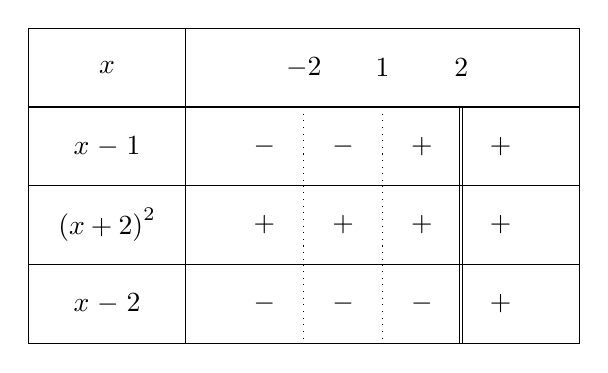
\begin{tikzpicture} 
			\tkzTabInit[lgt=2,espcl=1] 
				{$x$         /1, 
				$x-1$   /1, 
				$\left(x+2\right)^2$  /1,
				$x-2$       /1}% 
				{  , $-2$ , $1$ ,$2$,  }% 
			\tkzTabLine{ , - , t , - , t , + , d , + ,}
			\tkzTabLine{ , + , t , + , t , + , d , + ,}
			\tkzTabLine{ , - , t , - , t , - , d , +, }
		\end{tikzpicture} 

		We see from the chart that $\displaystyle \dfrac{(x-1)(x+2)^2}{x-2}$ will be negative in $(1,2)$.  At $x=-2$ and $x=1$ it is zero.
		The solution is then: $\left\{ -2\right\} \cup [ 1, 2 )$.
	\end{explanation}
\end{example}


\begin{problem}
	Find the solution of the inequality: $\displaystyle x + \dfrac{9}{x-1} > 5$.
	\begin{multipleChoice}
		\choice{$(1, \infty)$}
		\choice{$[1,\infty)$}
		\choice[correct]{$(1,2)\cup (2,\infty)$}
		\choice{$\{1\} \cup [2,\infty)$}
		\choice{none of the above}
	\end{multipleChoice}
\end{problem}


\begin{example}
	Solve the inequality
	\[ \frac{1}{x-2} - \frac{4}{x+1} \leq 3 \]
	\begin{explanation}
		We'll start by moving everything to the left-hand side and combining them into a single fraction.
		\begin{align*}
			\frac{1}{x-2} - \frac{4}{x+1} &\leq 3 \\
			\frac{1}{x-2} - \frac{4}{x+1} - 3 &\leq 0\\
			\frac{1(x+1)}{(x-2)(x+1)} - \frac{4(x-2)}{(x+1)(x-2)} - \frac{3(x+1)(x-2)}{(x+1)(x-2)} &\leq 0\\
			\frac{(x+1) - (4x-8) - (3x^2-3x-6)}{(x+1)(x-2)} &\leq 0\\
			\frac{-3x^2+15}{(x+1)(x-2)} &\leq 0\\
			\frac{-3(x^2-5)}{(x+1)(x-2)} &\leq 0
		\end{align*}
		To solve this, we'll construct a sign chart.  We start by noticing that $x^2-5 =0$ only if $x = \pm \sqrt{5}$.
		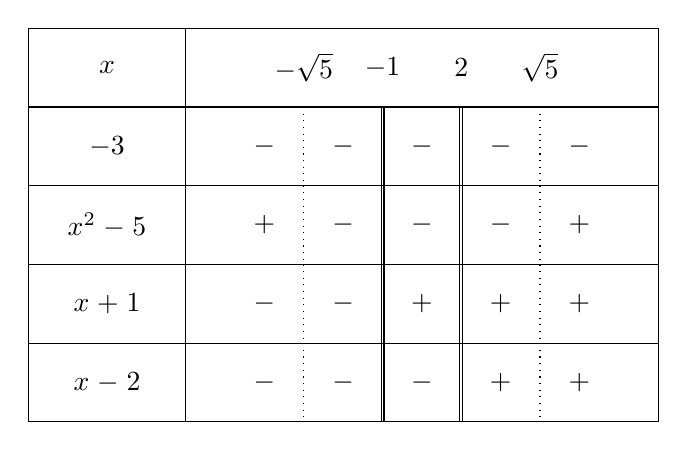
\begin{tikzpicture} 
			\tkzTabInit[lgt=2,espcl=1] 
				{$x$         /1, 
				$-3$    /1,
				$x^2-5$   /1, 
				$x+1$  /1,
				$x-2$       /1}% 
				{  , $-\sqrt{5}$ , $-1$ , $2$, $\sqrt{5}$,   }% 
			\tkzTabLine{ , - , t , - , d , - , d , - , t, -, }
			\tkzTabLine{ , + , t , - , d , - , d , - , t, +,}
			\tkzTabLine{ , - , t , - , d , + , d , +, t, +, }
			\tkzTabLine{ , - , t , - , d , - , d , +, t, +, }
		\end{tikzpicture} 
		
		We see from the sign chart, that the solution is $\displaystyle \left( -\infty, -\sqrt{5} \right] \bigcup \left(-1, 2\right) \bigcup \left[ \sqrt{5}, \infty \right)$.
	\end{explanation}
\end{example}







\end{document}
